\section{Background}\label{Sect:background}
\subsection{Linear Algebra}\label{Sect:linearAlgebra}
A basic knowledge of linear algebra, data analysis, and signal processing is required to understand how to build simple yet useful models. Samples from an unknown function are presented in Figure \ref{fig:func1Samples}. Building a function that matches the data will now be investigated.

\begin{figure}[h]
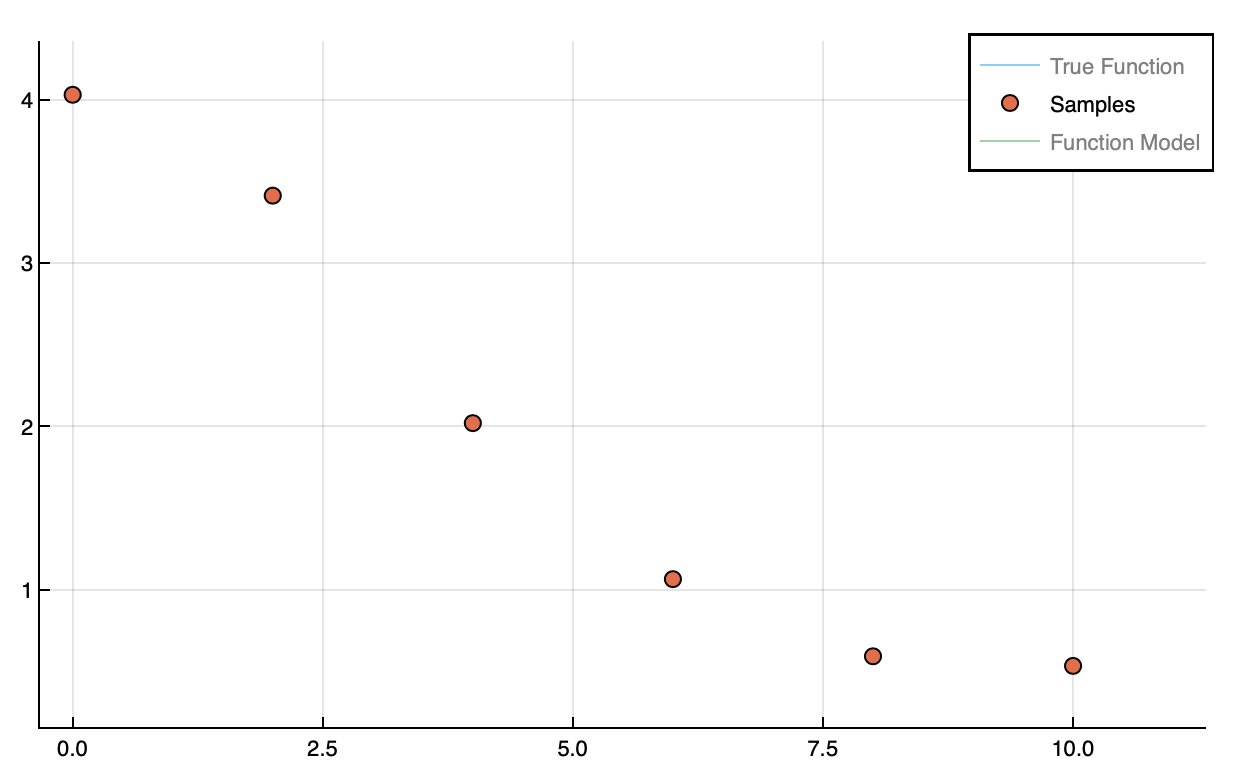
\includegraphics[scale = 0.4]{Figures/func1Samples}
\caption{An unknown function sampled by 6 data points.
\label{fig:func1Samples}} 
\end{figure}

\par It will be assumed that the function can be expanded using a basis, and in this case, a power series:

\begin{align}
f(x) &= \sum_{n=0}^\infty b_n x^n
	\label{eq:powerSum}\\ 
&= x^0b_0 + x^1b_1 + x^2b_2 + \ldots\ .
	\label{eq:powerSeries}
\end{align}

with the coefficients $b_n$ to be determined via the fitting process. Evaluating equation \ref{eq:powerSeries} at the observed data points in figure \ref{fig:func1Samples} produces a system of equations:

\begin{align}
f(0) &= b_0 \nonumber \\
f(2) &= b_0 + 2 b_1 + 4 b_2 + \dots \nonumber \\
f(4) &= b_0 + 4 b_1 + 16 b_2 + \dots \nonumber \\
f(6) &= b_0 + 6 b_1 + 36 b_2 + \dots \nonumber \\
f(8) &= b_0 + 8 b_1 + 64 b_2 + \dots \nonumber \\
f(10) &= b_0 + 10 b_1 + 100 b_2 + \dots\\
\end{align*}

This system of equations can be expressed in the following matrix form:

\begin{equation} \label{eq:LinAlgSubscript}
\begin{bmatrix}
1 & x_1 & x_1^2 & x_1^3 & x_1^4 \\
1 & x_2 & x_2^2 & x_2^3 & x_2^4 \\
1 & x_3 & x_3^2 & x_3^3 & x_3^4 \\
 & & \vdots & &
\end{bmatrix}
\begin{bmatrix}
b_0 \\
b_1 \\
b_2 \\
b_3 \\
b_4 
\end{bmatrix}
=
\begin{bmatrix}
f(x_1) \\ 
f(x_2) \\
f(x_3) \\ 
\vdots
\end{bmatrix}.
\end{equation}

And finally, $\mathbf{A}$ and $\vec{y}$ can be populated with their true values,

\begin{equation} \label{eq:realValues}
\begin{bmatrix}
1 & 0 & 0^2 & 0^3 & 0^4 \\
1 & 2 & 2^2 & 2^3 & 2^4 \\
1 & 4 & 4^2 & 4^3 & 4^4 \\
1 & 6 & 6^2 & 6^3 & 6^4 \\
1 & 8 & 8^2 & 8^3 & 8^4 \\
1 & 10 & 10^2 & 10^3 & 10^4
\end{bmatrix}
\begin{bmatrix}
b_0 \\
b_1 \\
b_2 \\
b_3 \\
b_4 
\end{bmatrix}
=
\begin{bmatrix}
f(0) \\ 
f(2) \\
f(4) \\ 
f(6) \\
f(8) \\
f(10)
\end{bmatrix}.
\end{equation}


The shape of the matrix $\mathbf{A}$ determines the type of solution that can be found.  If there are fewer equations (rows) than unknowns (columns), the system is underdetermined and if it has more rows than columns it is overdetermined.  


\subsubsection{Underdetermined systems}
Because the columns of an underdetermined system are linearly dependent, there are an infinite number of vectors $\vec{b}$ that can solve the system.  To arrive at a single vector, the solution must be constrained using some chosen criteria.  A commonly-used criteria is to minimize the $\ell_2$-norm of the solution vector. 

\par Solving an underdetermined system is done by using singular value decomposition (SVD)\cite{linAlg-book}. To solve $\mathbf{A}\vec{b}=\vec{y}$, first the eigenvalues and their corresponding orthonormal eigenvectors of $\mathbf{A}^T\mathbf{A}$ must be found. $V$ is the matrix containing these eigenvectors and $\Sigma$ is a diagonal matrix containing the singular values, the square roots of each non-zero eigenvalue, matching the shape of $\mathbf{A}$. Each column of the matrix $U$ can be constructed by $u_k=\frac{1}{\sigma_k}\mathbf{A}\vec{v_k}$ where $\sigma_k$ are the singular values and $\vec{v_k}$ are the columns of $V$. The final result is the complete SVD of $\mathbf{A}$ where $\mathbf{A}=U\Sigma V^T$ and $\vec{b}$ can be solved by,
\begin{align}
\mathbf{A}\vec{b} &= \vec{y} \label{eq:Aby} \\
\mathbf{A}^T\mathbf{A}\vec{b} &= \mathbf{A}^T\vec{y} \nonumber \\
\vec{b} &= (U\Sigma V^T)^T\vec{y} \nonumber \\
\vec{b} &= V\Sigma^TU^T\vec{y}.
\end{align}

\par The solution vector $\vec{b}$ is the well-known least squares solution to the system. Using this solution vector, the model can be used to make predictions of the function for any $x$ value within the range of sample points. To produce a continuous visual of the model's fit, the model can take in $x$ values for every point in the sample range and plot its respective evaluation. The result of this process can be seen in Figure \ref{fig:func1True}.

\subsubsection{Overdetermined system}
In an overdetermined system, since the column vectors don't span the space that they live in, there may be no vectors $\vec{b}$ that solve the system.  The ``closest" solution vector can be found by solving a slightly modified problem where the vector $\vec{y}$ is projected onto the subspace formed by the columns.  This is eqivalent to the well-known least squares approach and can be written in matrix form as:

\begin{align}
\mathbf{A}^T&(\vec{y} - \mathbf{A} \hat{\vec{b}}) = 0 \\
\mathbf{A}^T\vec{y} &= \mathbf{A}^T\mathbf{A}\hat{\vec{b}} \\
\hat{\vec{b}} &= (\mathbf{A}^T\mathbf{A})^{-1}\mathbf{A}^T\vec{y}, \label{eq:bSolve}
\end{align}
where $\mathbf{A}^T$ denotes the transpose of $\mathbf{A}$.

\par Since DFT data points are so costly to generate, the matrices that are typically encountered when building materials models are most-often underdetermined (i.e. more basis functions than data points).


\begin{figure}[h]
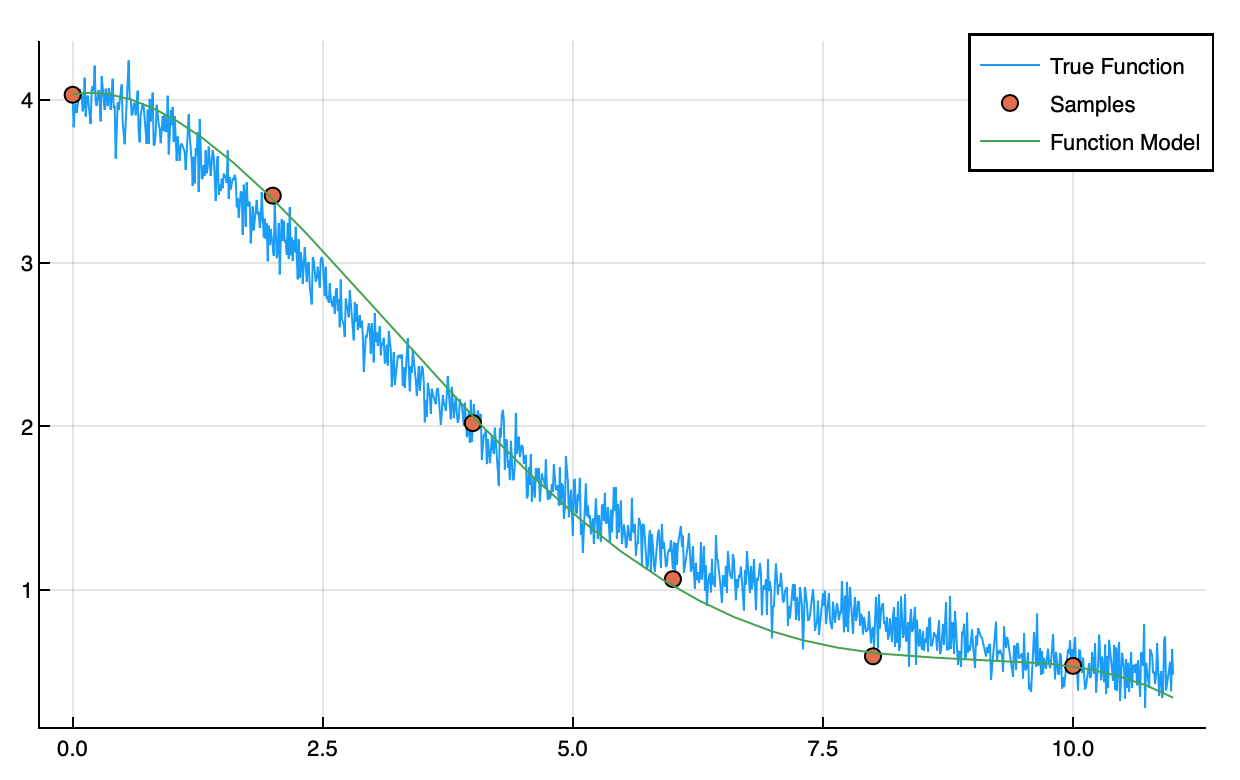
\includegraphics[scale = 0.4]{Figures/func1True}
\caption{The "Witch of Agnesi" function with Gaussian noise is shown in blue.  Samples from this function were gathered (circles) and used to construct a model using a simple polynomial basis.  The fit function is depicted in green.
\label{fig:func1True}} 
\end{figure}



\subsection{Basis Functions and Size of Training Set}\label{Sect:samplesAndFunctions}
\par The quality of the fit will be affected by (1)- the size of the training set (number of rows in matrix $\mathbf{A}$) and (2)- number of basis functions included in the expansion (columns in matrix $\mathbf{A}$). The convergence of our model with respect to these two parameters must be investigated. In theory there is no limit to the size of the training set or number of basis functions. However, since QM data is costly to generate, the size of the training set has a reasonable upper limit on the order of hundreds. In the example given, an increase in the traning set size or basis functions count will not dramatically affect the computational power required, but becomes a greater concern for models of systems with increasing complexity. 
\par As discussed, the number of basis functions can make a large impact, but another important factor is quality. Though the choice of basis functions in the example above was simple, it can often be a difficult choice. Consider, for example, a Fourier basis. The equivalent of Equation \ref{eq:LinAlgSubscript} in this basis would be

\begin{equation} \label{eq:fourierBasis}
\begin{bmatrix}
\sin(x_1) & \sin(2x_1) \\
\sin(x_2) & \sin(2x_2) & \ldots & \ldots \\
\sin(x_3) & \sin(2x_3) \\
\vdots & & \ddots & & \\
\sin(x_n) & \ldots & & \sin(mx_n)
\end{bmatrix}
\begin{bmatrix}
b_0 \\
b_1 \\
b_2 \\
\vdots \\
b_m 
\end{bmatrix}
=
\begin{bmatrix}
f(x_1) \\ 
f(x_2) \\
f(x_3) \\ 
\vdots \\
f(x_n)
\end{bmatrix},
\end{equation}
where $\mathbf{A}$ is an $n\times m$ matrix.
\par When used in the proper circumstance, this Fourier basis can be an excellent choice for modeling a function, as in Figure \ref{fig:2dFourier}.

\begin{figure}[h]
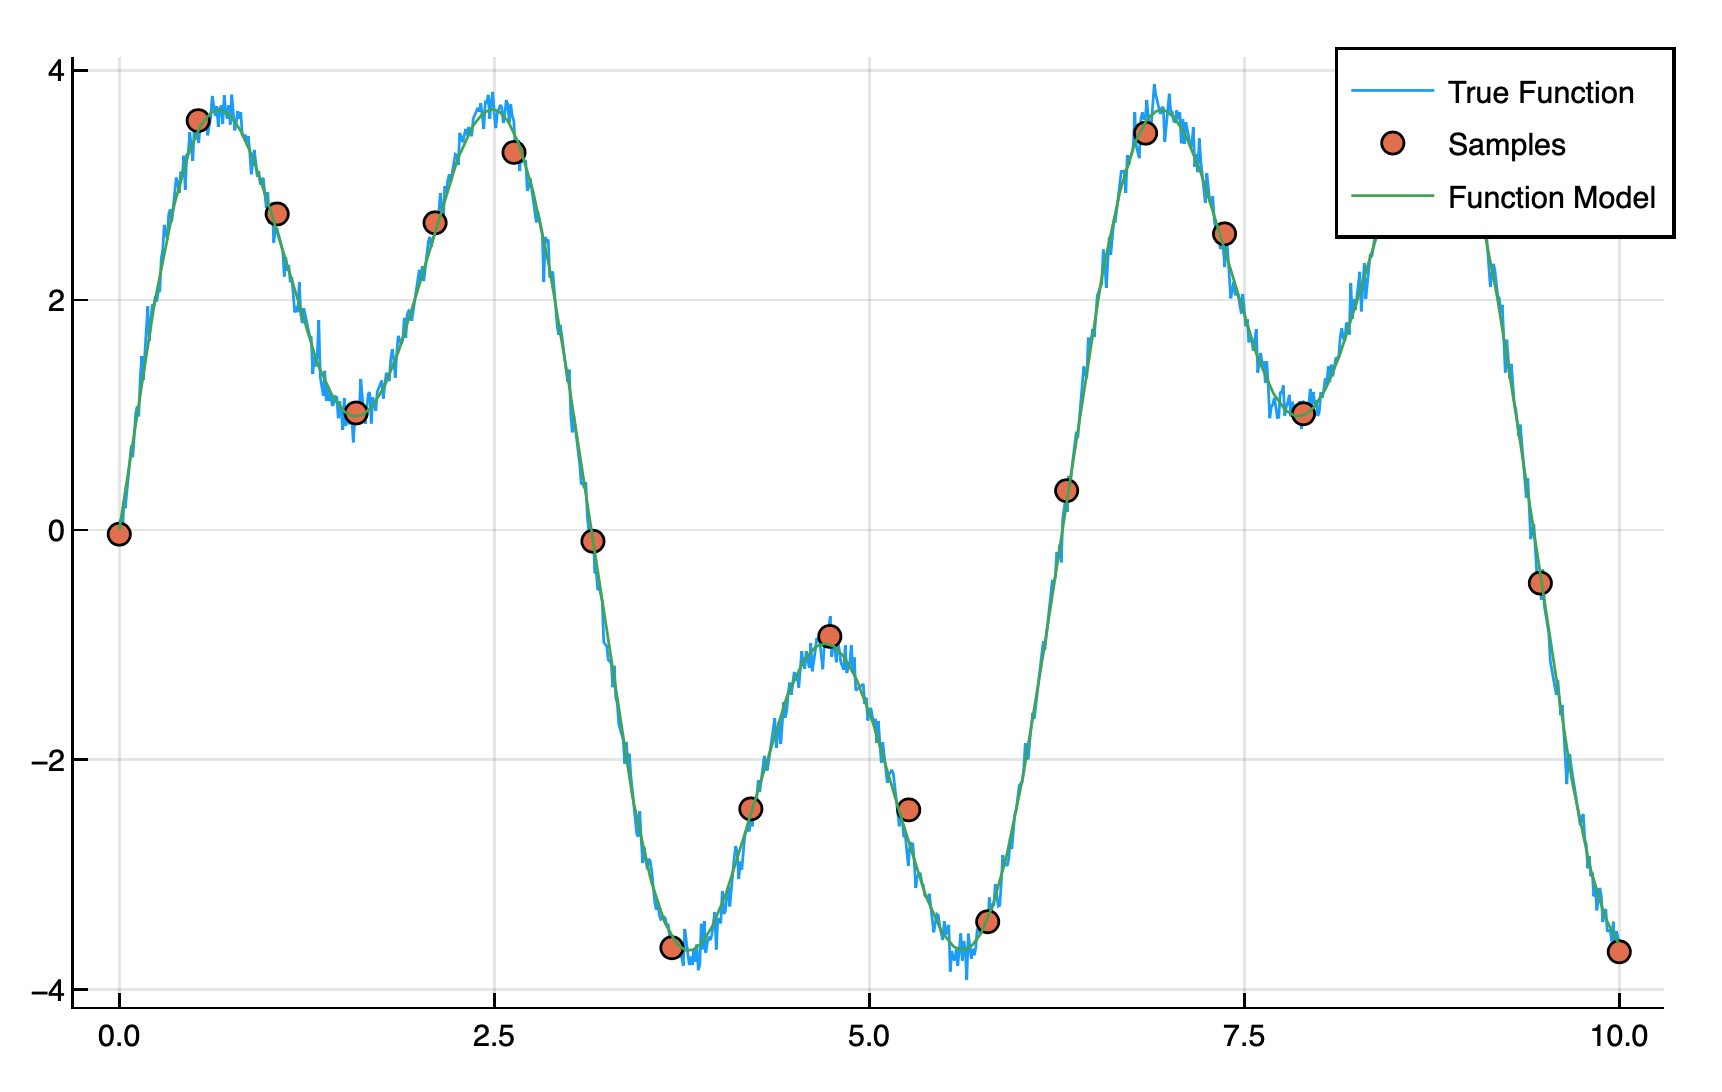
\includegraphics[scale = 0.27]{Figures/2dFourier}
\caption{The sample points shown were used to build a model of the function in green, and the true function is displayed in blue. The Fourier basis resulted in an excellent fit. 
\label{fig:2dFourier}} 
\end{figure}

\par When chosing sample points, there are again two variables to consider: number and breadth. As will be seen later, the number of samples can have a significant impact on the construction time and accuracy of a model. The breadth of samples is similarly important. If all samples from Figure \ref{fig:2dFourier} were taken between 0 and 1, the model produced would be a poor fit for the function, as in Figure \ref{fig:poorSamps}. 

\begin{figure}[h]
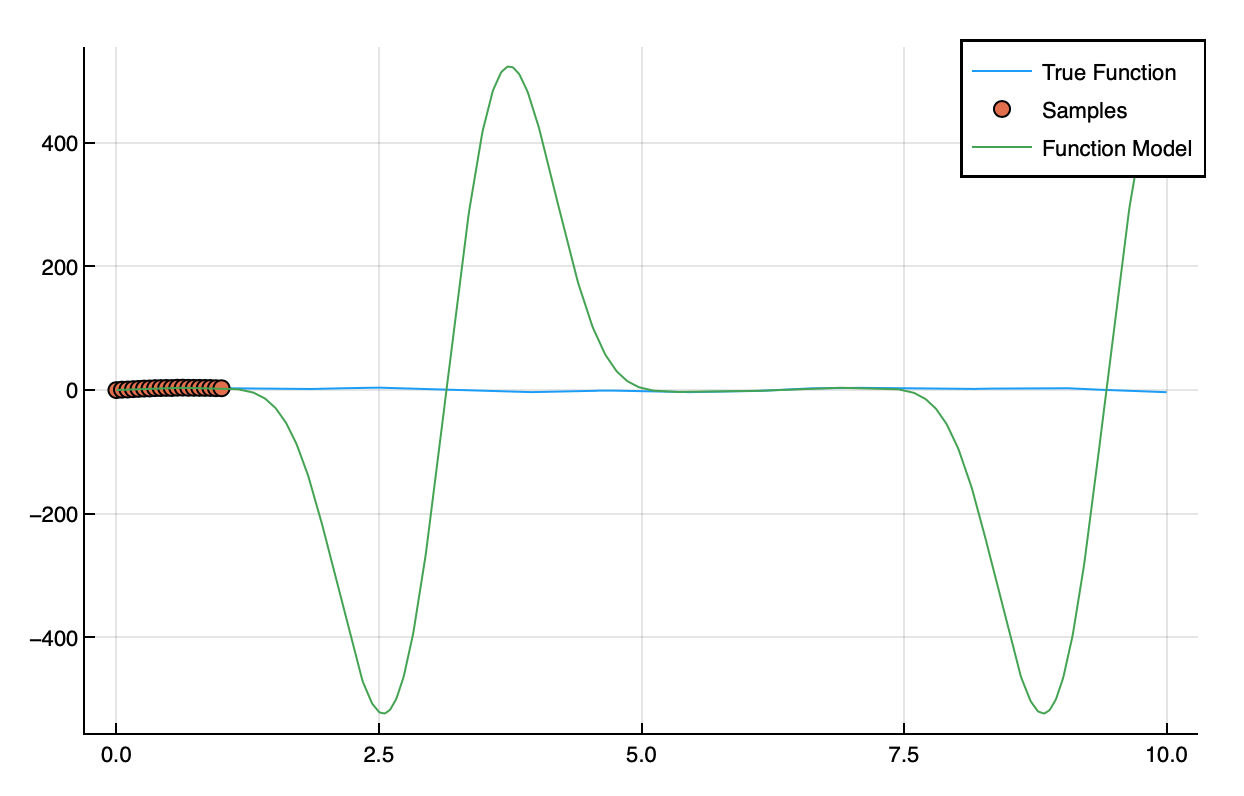
\includegraphics[scale = 0.4]{Figures/poorSamps}
\caption{Gathering samples that are not uniformly distributed across the function space will produce a model that does not predict well across the space. In this case, the secret function from Figure \ref{fig:2dFourier} was only sampled from the interval 0 to 1. If the model were evaluated at $x=2.5$, the fit would produce a highly inaccurate result when compared to the true function.
\label{fig:poorSamps}} 
\end{figure}

\par By this point it should be obvious to the reader that the decision of number and breadth of sample points as well as quantity and quality of basis functions is critical to the model's performance. With well chosen basis functions but poor breadth of samples, a model's accuracy can be greatly limited, as in Figure \ref{fig:poorSamps}. Figure \ref{fig:3dFourier} shows the reverse situation, good number and breadth of samples, but poorly chosen basis functions. 

%\begin{figure}[h]
%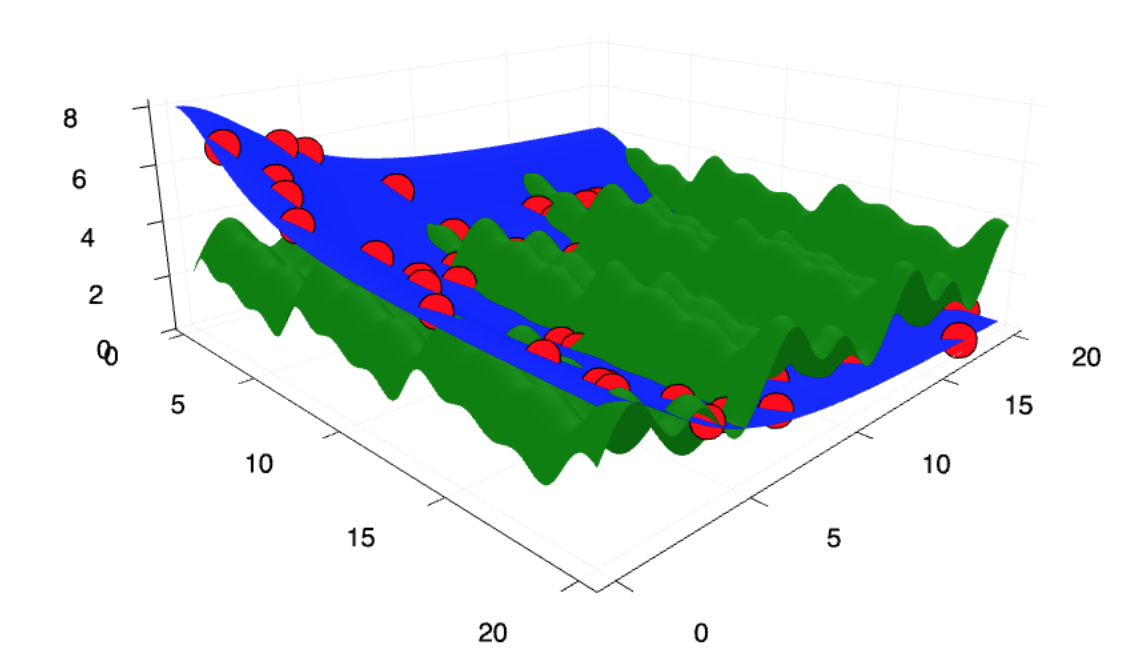
\includegraphics[scale = 0.42]{Figures/3dFourier}
%\caption{Choosing the right basis: The upper graph is a fit to a function of two variables using a Fourier basis.  The lower graph is a fit to the same function using a polynomial basis. The Fourier basis is unable to reproduce the true function whereas the polynomial basis can. The red points show the sampling of the true function. .
%\label{3dFourier}} 
%\end{figure}

\begin{figure}
  \begin{subfigure}{0.35\textwidth}
    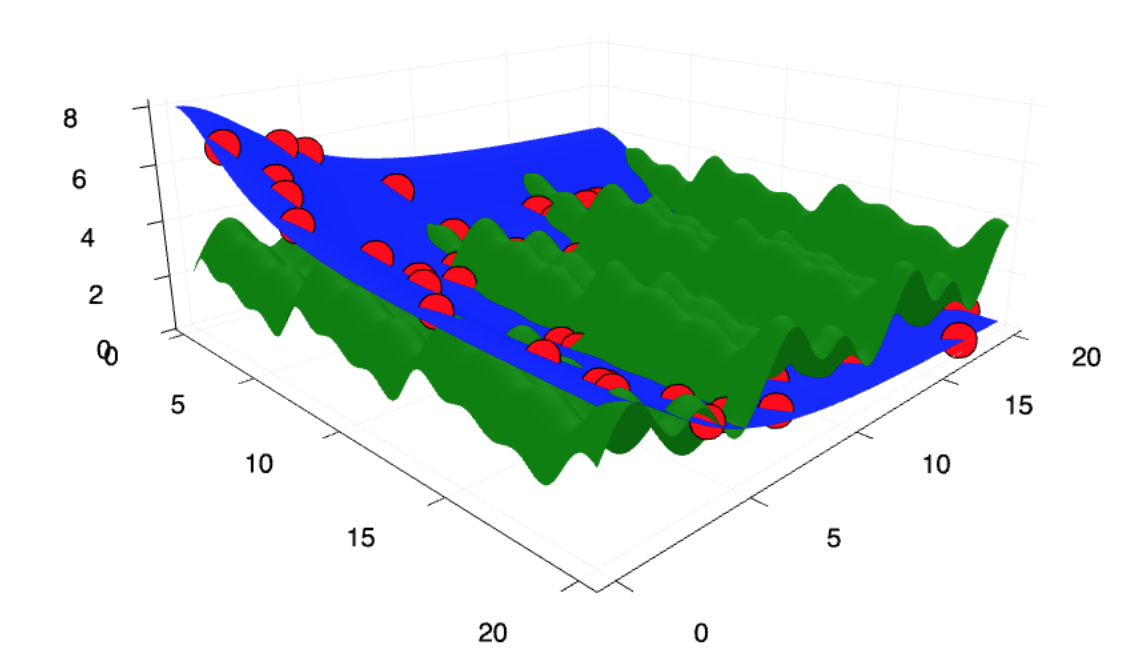
\includegraphics[width=\linewidth]{Figures/3dFourier}
    \caption{Fourier basis. $A$ is a $50\times7$ matrix.} 
    \label{fig:3dFourier}
  \end{subfigure}%
  \\
  \begin{subfigure}{0.35\textwidth}
    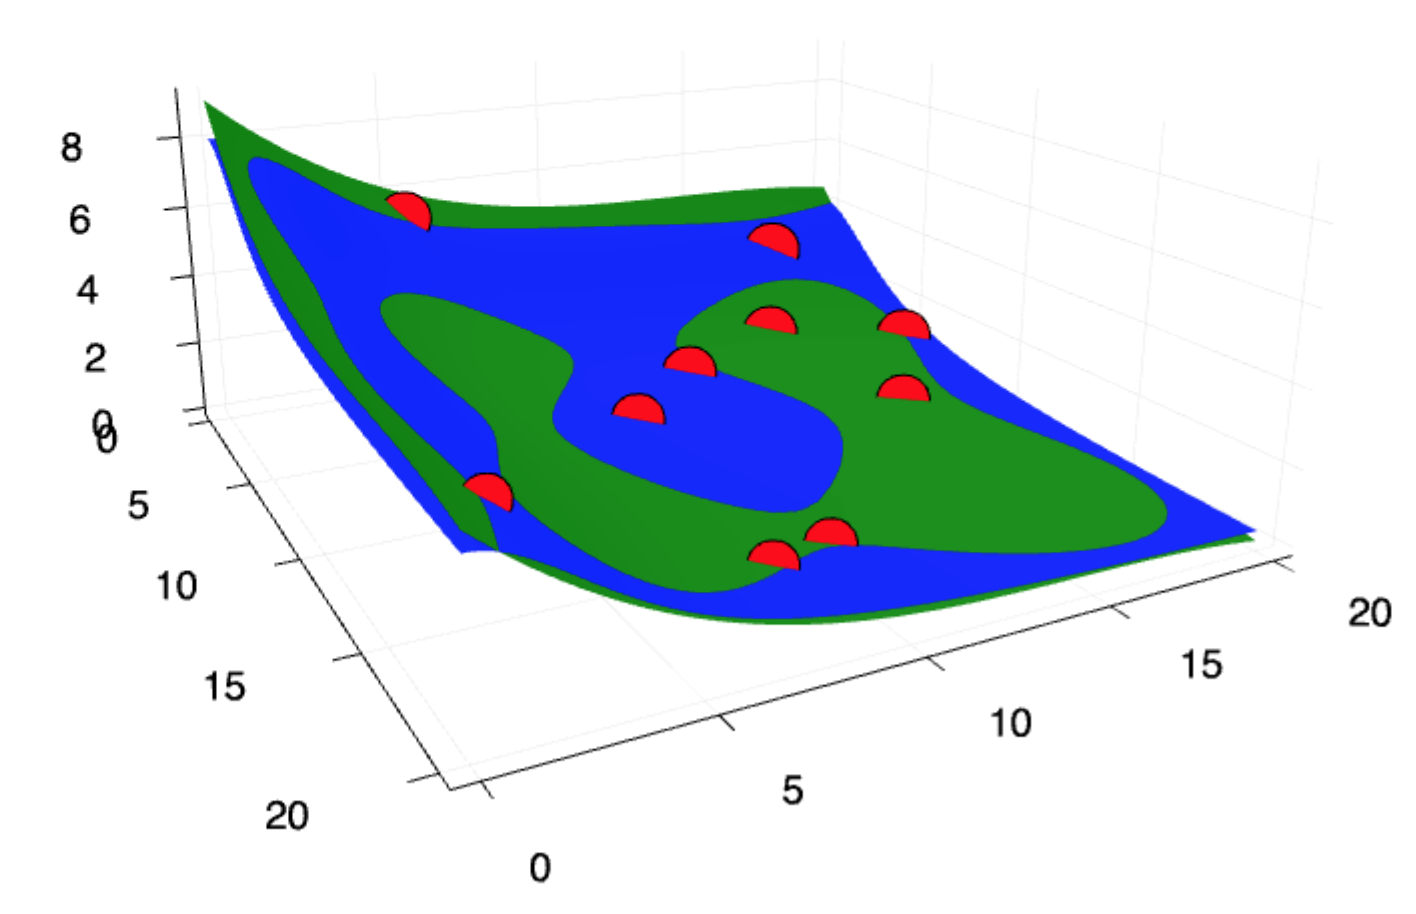
\includegraphics[width=\linewidth]{Figures/3dPower}
    \caption{Power basis. $A$ is a $10\times7$ matrix.} 
    \label{fig:3dPower}
  \end{subfigure}%
\caption{A three dimensional function in blue with a constructed model in green. The red points show the sampling of the true function. (a) In this case, a Fourier basis is a poor choice and resulted in an inaccurate model of the true function. (b) A Power series makes a convincingly better fit even with significantly fewer sample points.} \label{fig:3dFit}
\end{figure}


\subsection{Julia}\label{Sect:julia}
The figures provided throughout this paper were produced using the Julia programming language. Though encouraged to use Python for the majority of my formal education, Julia is a relatively new and fast growing language in terms of popularity. 
